\chapter{Analysis}
\section{Include Values}
calculated fron data, graphs, answers to Qs

\section{Average Time Calculated}
In the following data tables, the average time of the fall for each ball at 
each height is calculated

\begin{figure}[!h]
  \begin{minipage}{0.45\textwidth}
    \centering
    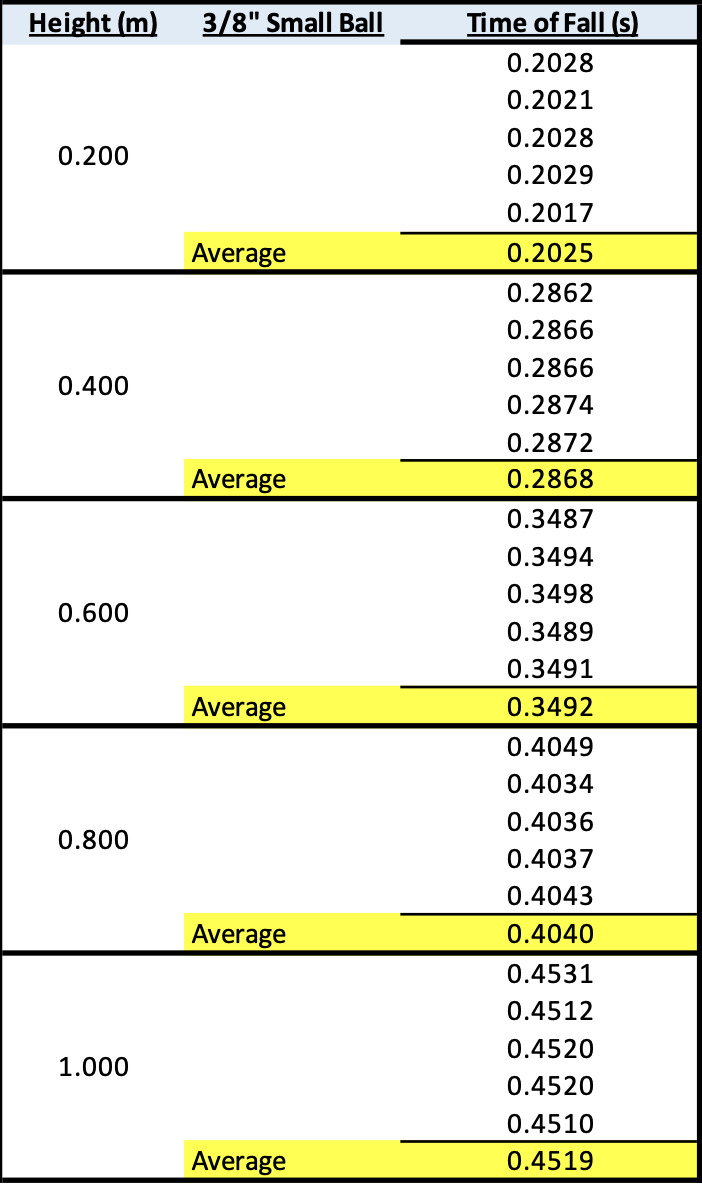
\includegraphics[scale=0.39]{resources/SmallTableAverage.jpg}
  \end{minipage}\hfill
  \begin{minipage}{0.45\textwidth}
    \centering
    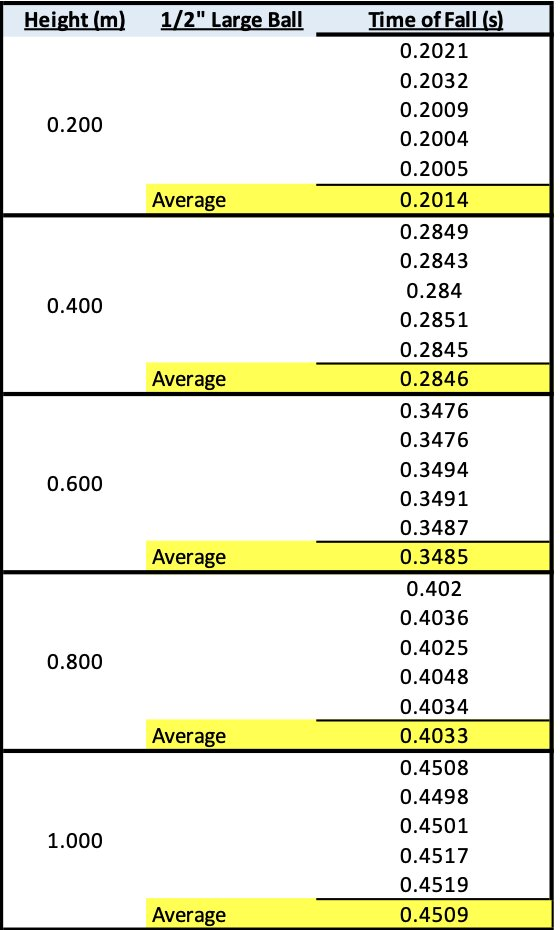
\includegraphics[scale=0.5]{resources/LargeAverageTable.jpg}
  \end{minipage}

\end{figure}


\newpage

\section{Graphed Data}
The following graphs for the small and large ball and their avaerge fall times
at each height squared then divided by 2, are plotted on a scatter plot and 
given a linear line with a calculated slope.


\begin{figure}[!h]
    \centering
    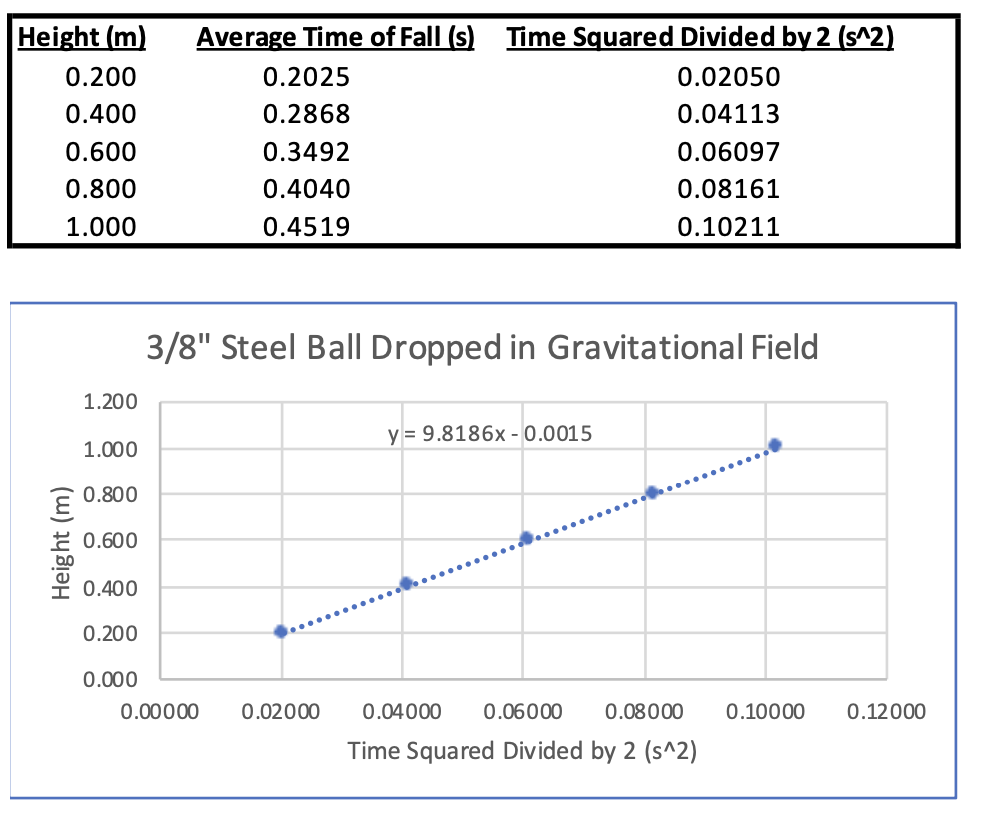
\includegraphics[scale=0.55]{resources/GraphSmall.png}
    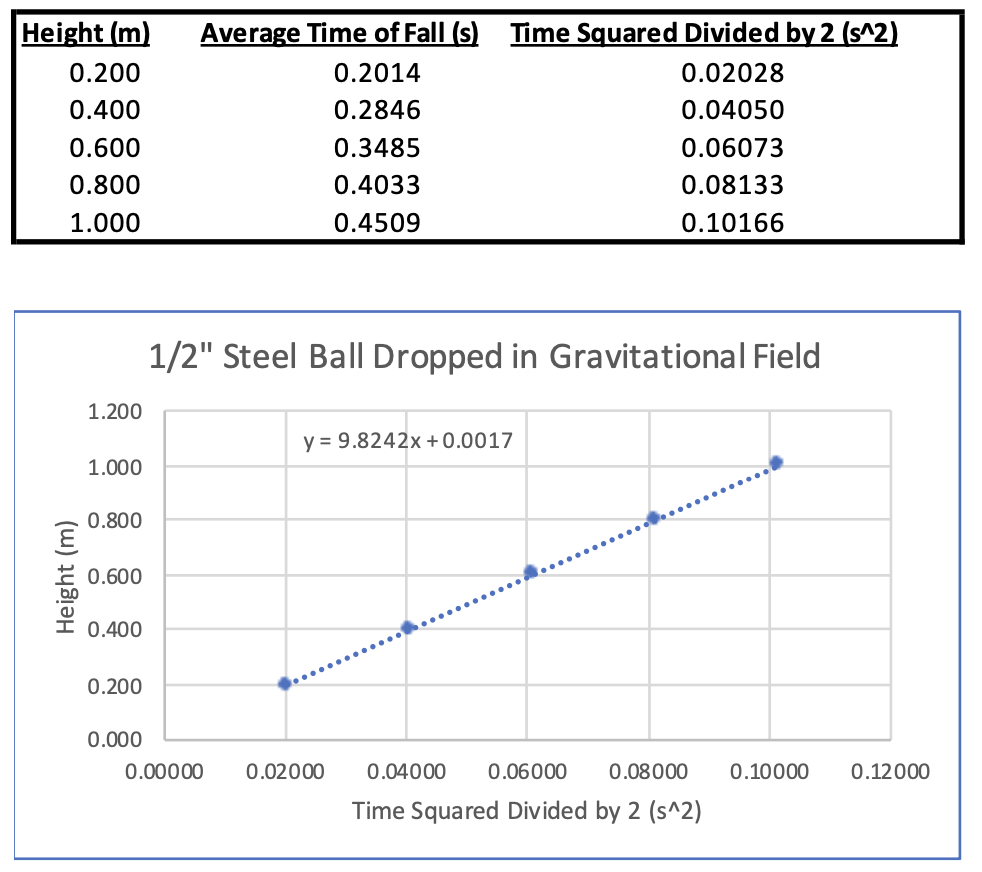
\includegraphics[scale=0.55]{resources/GraphLarge.png}
\end{figure}

\newpage
